% !TeX root = ../../../book.tex
\section{真理与证明}\label{sec:section1.1}

你怎么知道一件事是真还是假?比如,上学时老师告诉你三角形的内角和为 $180$ 度,但你怎么\emph{知道}这是真的呢?万一你遇到一个从未学过基础几何的外星人呢?你该如何\emph{说服}对方相信这一点呢?从某种程度上说,这就是数学:提出新的命题,以严谨的方式确定其真假,并向他人(甚至是外星人)解释这些发现。遗憾的是,似乎很多人认为数学家的工作就是整天计算大数的乘积;但事实上,数学远比通常认为的复杂算术更具创造性和写作性质。本书的目标之一,就是让你相信这一点,但这并非主要目的。本书的首要目标是向你揭示数学思维、解决问题和给出证明的真正内涵,教你掌握这些方法,并让你体会其中的乐趣!

顺便一提,你可能好奇``某事为真意味着什么''?要深入探讨这个问题,需要涉及哲学、心理学、甚至语言学领域,我们在此不做过多展开。然而就数学而言,其核心思想是:\textbf{只有能够}\emph{证明}\textbf{某事}\emph{永远}\textbf{成立它才为真}。我们知道 $1+1=2$ 永远为真。无论黑夜白昼,这个等式永远成立。(不过,你有没有想过如何证明它?实际上,证明这个问题非常困难!有本名为\emph{《数学原理》}的书从``第一性原理''出发,耗费了很多页的论证才最终得出 $1+1=2$!)这或许与其他科学领域完全不同。如果我们进行 $10$ 次物理实验并观测到相同的结果,能否断定它会\emph{永远}发生?做一百万次呢?十亿次呢?我们究竟在什么时候才算给出了\emph{证明}?在数学上,反复实验\emph{不能}构成证明!我们必须找到一个逻辑论证来解释为何现象必然发生。举个例子,数学中有一个著名的未解难题叫\href{https://baike.baidu.com/item/哥德巴赫猜想/72364}{哥德巴赫猜想}。至今无人知晓它是否正确,尽管计算机已将其验证到大约 $10^{18}$ 都成立。$10^{18}$ 是个\emph{极其巨大}的数字,但这仍不足以证明猜想是\textbf{真}是\textbf{假}。你看出区别了吗?数学家喜欢\emph{证明}事实,而不是用大量数值去检验,检验值只要未能覆盖\emph{全部}就\emph{不能}构成证明。

% !TeX root = ../../../book.tex
\subsection{三角迷思}\label{sec:section1.1.1}

在讨论证明的目标及其重要性时,我们引入了\textbf{证明}的概念。那么,如何\emph{定义}证明?这实际上是一个颇具挑战的问题!为逐步阐明这一概念,我们将给出若干数学论证案例。建议你仔细阅读,并思考它们是否具有说服力。它们\emph{证明}了什么?它们正确吗?是否正确?是否易于理解?阅读后有何感受?请先独立思考形成观点,然后再参考我们的分析。

我们给出的数学论证都与三角形有关。具体来说,都涉及\textbf{毕达哥拉斯定理}。

\begin{theorem}[毕达哥拉斯定理] \label{thm:pythagorean}
    在直角三角形中,若两直角边长分别为 $a$ 和 $b$,斜边长为 $c$,则 $a^2+b^2=c^2$。
\end{theorem}

\begin{center}
    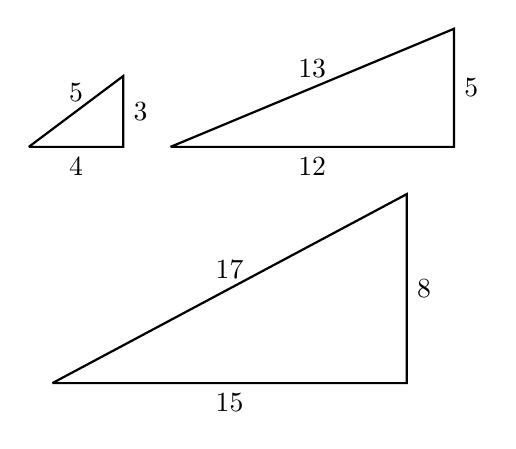
\begin{tikzpicture}[thick, scale=0.30]
        \draw (0,0) -- (4,0) node[midway,below]{$4$}
        -- (4,3) node[midway,right]{$3$}
        -- (0,0) node[midway,above]{$5$};
        \draw (6,0) -- (18,0) node[midway,below]{$12$}
        -- (18,5) node[midway,right]{$5$}
        -- (6,0) node[midway,above]{$13$};
        \draw (1,-10) -- (16,-10) node[midway,below]{$15$}
        -- (16,-2) node[midway,right]{$8$}
        -- (1,-10) node[midway,above]{$17$};
    \end{tikzpicture}
\end{center}

我们为何确信此定理成立?这个极其实用的结论,你可能在数学课堂上(或日常生活中不经意地)多次运用过。但你有没有思考过为什么这是真的?你会如何向持怀疑态度的朋友解释呢?这正是\textbf{数学证明}试图完成的:对事实给出清晰而严谨的解释。寻求证明背后的原因也十分有意义,它具有两重含义:即确保我们认为为真的事情确实为真,又避免要使用时进行重复论证。一旦(令人信服地)完成毕达哥拉斯定理的证明,后续只需引用定理名称即可;我们已经证明过了,所以无需再次证明。

那么,究竟什么构成了证明?如何判断解释是否足够清晰和简洁?一般来说,这些问题本身具有相当的复杂性,这也使得数学兼具科学与艺术的双重属性。尽管处理的都是严谨客观的事实,但如何有效地推理并以令人信服的方式呈现,实则是一门艺术。

\subsubsection*{``证明''范例}

让我们一起看几个``证明''的例子,看看它们是否足够好。(我们现在先说``证明'',稍后为其下更精确的定义。)这里是第一个:

\begin{proofs}{``证明'' 1.}
    构造边长为 $a+b$ 的正方形。在正方形内部放置 $4$ 个全等的直角三角形,形成边长为 $c$ 的内接正方形。

    \begin{center}
        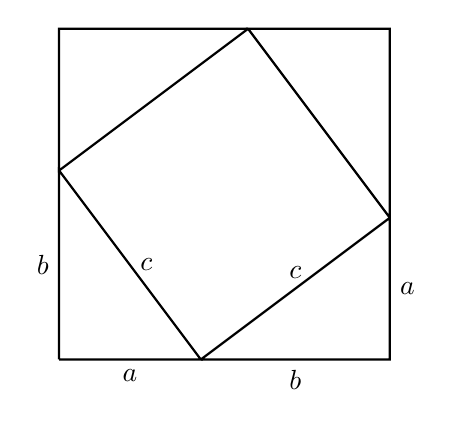
\begin{tikzpicture}[thick, scale=0.6]
            \draw (0,0) -- (3,0) node[midway,below]{$a$}
            -- (0,4) node[midway,right]{$c$}
            -- (0,0) node[midway,left]{$b$};
            \draw (3,0) -- (7,0) node[midway,below]{$b$}
            -- (7,3) node[midway,right]{$a$}
            -- (3,0) node[midway,above]{$c$};
            \draw (7,3) -- (7,7)
            -- (4,7)
            -- (7,3);
            \draw (4,7) -- (0,7)
            -- (0,4)
            -- (4,7);
        \end{tikzpicture}
    \end{center}

    大正方形的面积可以用两种方式表示:直接应用正方形的面积公式,或者把内接正方形和四个直角三角形的面积加起来。因此,下面这个等式一定成立。
    \[(a+b)^2=c^2+4\cdot\frac{ab}{2}=c^2+2ab\] 
    将左边表达式展开,然后两边同时消掉同类项可得 
    \[a^2+\cancel{2ab}+b^2=c^2+\cancel{2ab}\] 
    所以,$a^2+b^2=c^2$ 成立。
\end{proofs}

上面的证明是否具有说服力?每一步是否合理?可能你现在还太不确定,那么让我们接着看一下此定理的另一种``证明''。

\begin{proofs}{``证明'' 2.}
    假设毕达哥拉斯定理成立。绘制直角三角形,并过直角顶点向对应边做高。如下图所示:
    \begin{center}
        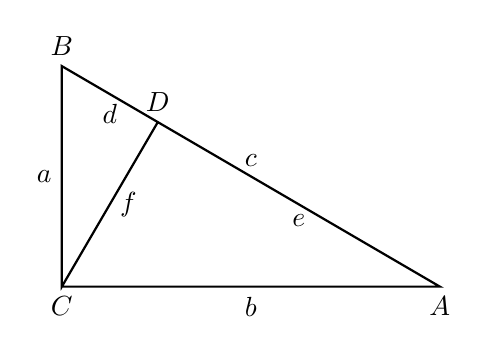
\begin{tikzpicture}[thick, scale=0.8]
            \coordinate (C) at (0,0);
            \coordinate (A) at (6,0);
            \coordinate (B) at (0,3.5);
            \coordinate (D) at (1.523316, 2.611399);
            \draw (C) node[anchor=north]{$C$}
            -- (A) node[anchor=north]{$A$} node[midway,below]{$b$} 
            -- (B) node[anchor=south]{$B$} node[midway,above]{$c$}
            -- (C) node[midway,left]{$a$}
            -- (D) node[anchor=south]{$D$} node[midway,right]{$f$}
            -- (A) node[midway,below]{$e$} 
            -- (D)
            -- (B) node[midway,below]{$d$};
            \rightAngle{B}{D}{C}{0.3};
        \end{tikzpicture}
    \end{center}
    因为毕达哥拉斯定理成立,所以我们可以将其应用到图中的三个直角三角形中,即三角形 $ABC, BCD, ACD$。(定义 $e = c-d$)可得
    \begin{align*}
        a^2 &= d^2 + f^2 \\
        b^2 &= f^2 + e^2 \\
        c^2 &= a^2 + b^2
    \end{align*}
    将前两个方程相加,再用代入第三个方程,可得
    \[c^2 = d^2 + e^2 +2f^2\]
    注意到 $\angle ABC$ 与 $\angle ACD$ 相等,因为它们都与角 $\angle CAB$ 互余,由此可知 $\triangle CDB$ 与 $\triangle ADC$ 相似。(此处默认你对平面几何有所了解。)由此可得 $\frac{e}{f} = \frac{f}{d}$,因此 $f^2 = ed$。我们可以将其带入上面的公式替换 $f^2$,结果如下:
    \[c^2 = d^2+e^2+2de = (d+e)^2\]
    两边同时开方(已知 $c,d,e$ 都是正数)可得 $c = d+e$,根据边长 $d$ 和 $e$ 的定义,这显然成立。因此,假设毕达哥拉斯定理成立是正确的。
\end{proofs}

这个证明怎么样?有说服力吗?表述清晰吗?在确定什么构成``正确的''或``良好的''证明之前,让我们再考察一个``证明''。

\newpage

\begin{proofs}{``证明'' 3.}
    观察下图
    \begin{center}
        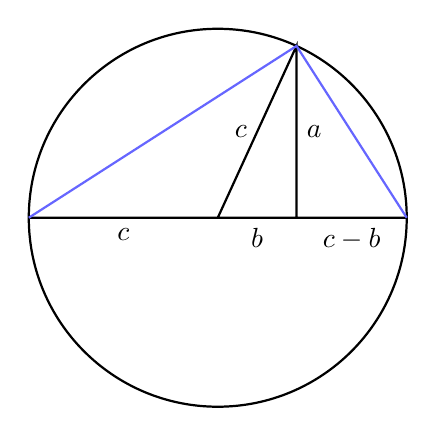
\begin{tikzpicture}[thick, scale=0.4]
            \coordinate (O) at (0,0);
            \coordinate (A) at (-6,0);
            \coordinate (B) at (6,0);
            \coordinate (C) at (2.5,0);
            \coordinate (D) at (2.5,5.45435);
            \draw (O) circle (6);
            \draw (A) -- (O) node[midway,below]{$c$}
            -- (C) node[midway,below]{$b$}
            -- (B) node[midway,below]{$c-b$}
            -- (C)
            -- (D) node[midway,right]{$a$}
            -- (O) node[midway,left]{$c$};
            \draw[color=blue!60] (A) -- (D) -- (B);
            \rightAngle{B}{C}{D}{0.6};
        \end{tikzpicture}
    \end{center}  
    由图形可得 $\frac{a}{b+c} = \frac{c-b}{a}$,因此 $a^2 + b^2 = c^2$。
\end{proofs}

这个证明对你来说合理吗?最后,还有一个需要思考的``证明''。

\begin{proofs}{``证明'' 4.}
    毕达哥拉斯定理必然成立,否则我的老师一直在欺骗我。
\end{proofs} 

\subsubsection*{讨论}

在继续阅读之前,建议你先独立思考这四个``证明'',也可与同学或朋友讨论一下。你认为什么构成``正确''的证明?清晰性和易读性重要吗?它会影响证明的``正确性''吗?

从历史角度看,数学证明的撰写历经多年演变,已经对什么构成``正确''的证明形成了普遍共识:

\begin{itemize}
    \item 从数学角度来说,证明中的每一\emph{步}、每一个逻辑推理和命题均需保持\emph{数学有效性},这一点非常重要。
    \item 同样重要的是,证明撰写者需(合理地)阐明陈述如何源于前置工作或外部知识。
\end{itemize}

这种对\emph{真理性}的要求,使得已建立的数学论证,可以通过逐步验证确认每个命题是\textbf{对}还是\textbf{错}。难点在于对清晰表达的界定。某种程度上,这就像最高法院大法官波特·斯图尔特(Justice Potter Stewart)对淫秽的著名定义:``见之即明''。

下面从清晰性和正确性两方面评估这四个论证:

\textbf{清晰性:}

\begin{itemize}
    \item ``证明'' 1 和``证明'' 2 表述清晰。明确解释了操作动机与依据。不仅给出了每个方程式的来源,还辅以图示说明。
    
    请注意,``证明'' 1 确实依赖一些基本的先验知识,例如基本代数运算以及三角形和正方形的面积公式,但这没有问题。

    同样地,``证明'' 2 依赖相似三角形的一些知识以及它们边长之间的关系。撰写者明确指出了这一点,所以有兴趣的读者可以查阅相关知识点。如果撰写者没有指出,读者可能会感到困惑,不知道如何得出这个结论。
    \item ``证明'' 3 写得非常糟糕!它没有提供任何解释。这使得读者很难确定其结论是否正确。尽管其中包括一张图片,但并没有解释\emph{为什么}要画一个三角形的外接圆,或者为什么能从图中得出所述方程。
    \item ``证明'' 4 虽语法正确,但并未提供任何\emph{解释}!
\end{itemize}

由此可见,对于一个逻辑正确且书写良好的证明来说,``证明'' 4 无疑是一个糟糕的证明。``证明'' 1 和``证明'' 2 仍在候选之列,因为它们至少写得很清楚。``证明'' 3 目前看可能不是一个好的证明;也许它确实包含正确的结论,只是需要更好的解释。通过重写可以使其变成一个良好的\emph{证明}。

让我们再来分析一下这四个论证的逻辑正确性:

\textbf{正确性:}

\begin{itemize}
    \item ``证明'' 1 大部分都很好。正确应用了正方形和三角形的面积公式,并且其代数运算也正确。但是我们怎么知道其所描述的过程 —— 将给定四个三角形放入正方形内 —— 会构建一个边长为 $c$ 的内接正方形?证明中只是说这样\emph{可以},但并未真正说明\emph{为什么可以}。不过,除此疏漏外,这个证明写得很好而且是正确的。
    
    (你能证明里面的形状实际上是正方形吗?看一下它的角度:你能说明为什么它们都是直角吗?)
    \item 很遗憾,``证明'' 2 完全是错误的!尽管它所做的每一个逻辑步骤都遵循前一个步骤。例如,假设我们以这种方式设置三角形,我们可以正确推断出 $\triangle CDB$ 和 $\triangle ADC$ 是相似三角形。然而,为什么我们可以在一开始就\emph{假设}该定理为\textbf{真}呢?总的来说,这不正是我们在证明中试图实现的目标吗?这是一个关键缺陷。\textbf{假设一个事实并从中推断出某些结论为真并不能得出原始假设必然为真。}
    
    如果这种方法有效,我们可以``证明''任意命题!举个例子:你如何看待以下证明 $0 = 1$ 的``证明''?
    \begin{proof}
        假设 $0 = 1$。那么,根据 $=$ 的对称性,$1 = 0$ 也是成立的。将这两个方程相加可得 $1 = 1$,这显然为真。因此,$0 = 1$ 是一个有效的假设,因此它一定为真。
    \end{proof}
    你看出上面证明与``证明'' 2 有什么相似之处吗?它们使用了同样有缺陷的推理:假设一个事实,做了一些工作得到我们已知为真的其他事实,然后断言假设的事实也必然为真。
    \item 对于``证明'' 3 ,大多数数学家会说这是一个``糟糕的证明'',尽管其透露出的结论似乎都是正确的。我们说``透露出''是因为,如果没有任何文字解释思路,就无从知晓撰写者想表达什么!然而,不得不说,完美证明的核心思路就包含其中。
    
    从图中,你可以证明方程 $\frac{a}{c+b} = \frac{c-b}{a}$ 一定成立。(提示:使用相似三角形!)进而可以推导出 $a^2 + b^2 = c^2$。

    你能写一些文字来配合图形,将其改写为良好的证明吗?
    \item 最后,几乎每个逻辑正常的人(我们希望如此!)都会说``证明'' 4 根本不是一个证明,无论做出这样的陈述多么方便。
\end{itemize}

综上,``证明'' 1 是一个良好的证明。在 4 个证明中,``证明'' 1 写得最清楚,逻辑也最正确。我们可以将其视作\textbf{证明}。``证明'' 2 是完全错误的,尽管它表述得非常清楚。``证明'' 3 包含正确的思路,但缺乏清晰的表述。``证明'' 4 离证明十万八千里,毫无讨论价值。

\subsubsection*{问题}

在继续讨论其他主题之前,留下一个问题供你思考:给定三个正数 $a,b,c$ 满足 $a^2+b^2=c^2$,是否一定存直角边长为 $a,b$ 斜边长为 $c$ 的直角三角形?倘若存在,你会如何着手构造它?若不存在,原因何在?


% !TeX root = ../../../book.tex
\subsection{质数时间}\label{sec:section1.1.2}

当我们讨论证明这个主题时,让我们看一下另一个重要定理的证明。首先简要回顾\emph{质数}的定义。

\subsubsection*{定义、示例与应用}

\begin{definition}\label{def:prime}
    若正整数 $p>1$ 的正因子只有 $1$ 和 $p$ 本身,则称 $p$ 为\dotuline{质数}。非质正整数称为\dotuline{合数}。
\end{definition}

质数在数学的诸多分支中都具有核心地位,而不仅限于研究整数性质的\textbf{数论}领域。数学中最著名的\textbf{猜想}(迄今为止既没有被证明也没有被证伪的命题)当数\emph{黎曼猜想}。该猜想已被证实与质数在整数中的分布规律密切相关,相关研究著作浩如烟海。此外,大多数现代密码学的基础都是大质数的乘积特性 —— 将两个大质数相乘容易,但将乘积逆向分解为两个大质数却极为困难。现在你知道了:每当你用信用卡在 iTunes 上购买歌曲时,背后的计算机系统都会将两个大质数相乘!

前几个质数依次为 $2, 3, 5, 7, 11, 13, 17, 19, 23,\dots$(注意,$1$ 不满足定义)。那么质数有多少个?相邻质数相距多远?是否存在分布规律?这些问题虽引人入胜却极难解答(有时甚至是不可能的!)。本节将聚焦其中一个问题:质数是否有无穷多个?

\subsubsection*{定理与证明}

\begin{theorem}[质数无穷性]
    质数有无穷多个。
\end{theorem}

\begin{proof}
    假设质数有有限多个,按升序列出为:$p_1, p_2, p_3, \dots, p_k$,所以 $p_k$ 为最大质数。现构造新数
    \[N = (p_1 \cdot p_2 \cdot p_3 \cdot \dots \cdot p_k) + 1\]
    $N$ 必有质因子。然而,它一定不能被 $p_1$ 或 $p_2$ 或 $\dots$ 或 $p_k$ 整除,因为根据 $N$ 的定义,除以上述质数都会得到余数 $1$。因此 $N$ 可以被列表中未列出的其他质数整除。

    如果 $N$ 是合数,那么我们就发现了一些新质数 $p < N$,它不在所有质数列表中。
    
    如果 $N$ 是质数,那么我们就得到了一个新质数 $N > p_k$,所以 $p_k$ 实际上并不是最大的质数。无论哪种情况,我们必然有一个新的质数不在给定的 $k$ 个质数的列表中,这与有限性假设矛盾。因此,质数必定有无穷多个。
\end{proof}

对于这个``证明''你怎么看?是否令你信服?这里的论证方式与我们迄今为止看到的其他论证方法有所不同。不妨尝试向同学解释本节的证明与上一节毕达哥拉斯定理的``证明 1''有何不同。我们很快将揭示:此处的``证明''实际上是一个完全正确的\emph{证明}!


% !TeX root = ../../../book.tex
\subsection{无理取闹}

现在让我们讨论另一类数字:\textbf{有理数}。你可能知道``分数''、``商''或``比率''指的都是有理数。

\subsubsection*{定义与示例}

以下是\emph{有理数}的精确定义:

\begin{definition}
    实数 $r$ 是\dotuline{有理数}当且仅当它可以表示为两个整数之比 $r = \frac{a}{b}$,其中 $a$ 和 $b$ 均为整数(且 $b \ne 0$)。

    一个实数不是有理数就是\dotuline{无理数}。
\end{definition}

定义并未规定有理数必须具有唯一的表示形式;它只要求有理数至少有一种定义中的表示。例如,$1.5$ 是有理数,因为 $1.5 = \frac{3}{2} = \frac{12}{8} = \frac{30}{20}$ 等等。这一定义具有完备性:一个实数不是有理数就是\textbf{无理数},\emph{非}有理数,即不存在将其表示为整数之比的形式。你可能知道 $\sqrt{2}$ 是一个无理数,但如何\emph{证明}这一点呢?请尝试自行证明。我们稍后会重新讨论这个问题(见示例 \ref{sec:section4.9.4})。其他常见的无理数还包括 $e, \pi, \varphi$ 以及 $\sqrt{n}$(其中 $n$ 为正整数且不为完全平方数)。

\subsubsection*{问题}

基于有理数/无理数的定义,我们可以探讨无理数的组合能否产生有理数。请尝试独立解答以下问题:若答案为``是'',请举例说明;若答案为``否'',请解释其不可能性。

\begin{enumerate}
    \item 是否存在无理数 $a$ 和 $b$ 使得 $a \cdot b$ 为有理数?
    \item 是否存在无理数 $a$ 和 $b$ 使得 $a + b$ 为有理数?
    \item 是否存在无理数 $a$ 和 $b$ 使得 $a^b$ 为有理数?
\end{enumerate}

你能构造出具体例子吗?事实上,这三个问题的答案均为``是''!前两问较为简单,第三问则略微棘手。

以下我们给出第三问的证明。有趣的是,该证明并不直接给出满足条件的 $a$ 和 $b$;而是将可能性缩小至两种情形,并证明其中\emph{必有}一种成立。听起来很有趣,对吧?我们来试试吧。

\begin{proof}
    已知 $\sqrt{2}$ 为无理数。考虑数字 $x = \sqrt{2}^{\sqrt{2}}$。有两种可能的情况:
    \begin{itemize}
        \item 若 $x$ 为有理数,则令 $a = \sqrt{2}, b = \sqrt{2}$ 即满足条件。
        \item 若 $x$ 为无理数,则令 $a = \sqrt{2}^{\sqrt{2}}, b = \sqrt{2}$,此时
        \[a^b = \Bigg(\sqrt{2}^{\sqrt{2}}\Bigg)^{\sqrt{2}} = \Big(\sqrt{2}\Big)^{\sqrt{2} \cdot \sqrt{2}} = \Big(\sqrt{2}\Big)^2 = 2\]
        $2$ 为有理数。
    \end{itemize}
    无论何种情形,均可找到无理数 $a$ 和 $b$ 使得 $a^b$ 为有理数。因此,这样的数字对必然存在。
\end{proof}

你觉得这个证明怎么样?是否有说服力?它以明确的``是''回答了上面的第三问,但未指明具体\emph{哪一对} $a, b$ 是正确的,而是告诉我们其中必有一对满足。(事实证明 $\sqrt{2}^{\sqrt{2}}$ 确为无理数,但这一事实需要额外证明。)

还有很多其他具体例子可以回答这个问题。你能想出任何其他方法吗?(提示:尝试使用 $\log_{10}$ 函数……)
